\documentclass{beamer}
\let\Tiny=\tiny

\usepackage{mathtools}
\usepackage{amsfonts}
\usepackage{amsmath}
\usepackage{graphicx}
\usepackage{pdfpages}
\usepackage[]{xcolor}
\usepackage{tikz}



\newcommand{\meo}[1]{\texttt{#1}} % My Eyes Only: notes just for me
\newcommand{\bigo}{\mathcal{O}}
\newcommand{\extra}[1]{{\color{purple} {#1}}}

\usetheme{default}
\usecolortheme{beaver}
\usefonttheme{serif}

\setbeameroption{show notes}

\newif\ifpresstime
	\presstimefalse
	\presstimetrue

\ifpresstime
		\renewcommand{\meo}[1]{}
		\date{April 13, 2018}
		\setbeameroption{hide notes}
	\else
		% \setbeameroption{show notes}
		\setbeameroption{show only notes}
		\date{\today}
	\fi

\usetikzlibrary{arrows, automata, shapes}


\title{Kleene's Theorem}
\author{James McFeeters}
\institute {Beloit College}
\begin{document}

\frame{
	\titlepage
}

\begin{frame}
	\frametitle{Basic Definitions}
	\begin{itemize}
		\item Symbol
		\pause
		\item Alphabet ($\Sigma$)
		\pause
		\item String / word
		\pause
		\item Language
	\end{itemize}
\end{frame}

\begin{frame}
	\frametitle{Building a Finite Automaton}
	\centering
	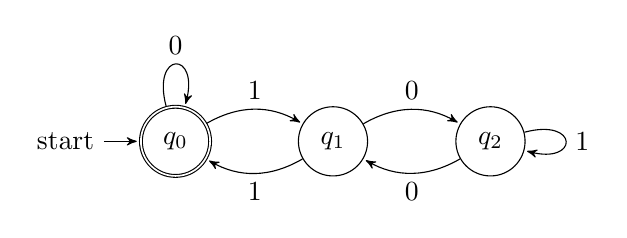
\begin{tikzpicture}[>=stealth',shorten >=1pt,auto,node distance=2cm]
		\node[initial,state,accepting] (q0)                {$q_0$};
		\node[state]                   (q1) [right of = q0] {$q_1$};
		\node[state]                   (q2) [right of = q1] {$q_2$};

		\path[->] (q0) edge [loop above] node {0} (q0);
		\path[->] (q0) edge [bend left]  node {1} (q1);
		\path[->] (q1) edge [bend left]  node {0} (q2);
		\path[->] (q1) edge [bend left]  node {1} (q0);
		\path[->] (q2) edge [bend left]  node {0} (q1);
		\path[->] (q2) edge [loop right] node {1} (q2);
	\end{tikzpicture}

\end{frame}
\note[itemize]{
	\item note
}


\begin{frame}[allowframebreaks]
	\frametitle{References}
	\bibliographystyle{amsplain}
	\nocite{*}
	\bibliography{../paper/references.bib}
\end{frame}

\end{document}
